\documentclass[conference]{IEEEtran}

\usepackage{amsmath, amssymb, amsfonts}
\usepackage{graphicx}
\usepackage{cite}
\usepackage{booktabs}
\usepackage{hyperref}
\usepackage{url}
\usepackage{algorithm}
\usepackage{algpseudocode}
\usepackage{tikz}
\usetikzlibrary{positioning, shapes, arrows.meta, calc, fit, backgrounds, shadows}
\usepackage{fontawesome5} % For the icons

\title{Sponge Attacks Against AI-Based Models in the Smart Grid: Analysis and Experimentation}

\author{\IEEEauthorblockN{Bora Pilav}
\IEEEauthorblockA{Institute for Automation and Applied Informatics (IAI)\\
Karlsruhe Institute of Technology\\
Karlsruhe, Germany\\
Email: ugglf@student.kit.edu}
}

\markboth{Seminar on Adversarial Machine Learning}{Sponge Attacks in Smart Grids}

\begin{document}
\maketitle

\begin{abstract}
The integration of Artificial Intelligence (AI) into the Smart Grid is critical for optimizing energy distribution, forecasting demand, and detecting anomalies in real-time. However, the deployment of these complex models introduces significant security vulnerabilities. While traditional adversarial attacks target model integrity to induce misclassifications, this report investigates ``Sponge Attacks''—a class of denial-of-service (DoS) attacks targeting model availability. Sponge attacks exploit the computational density of deep learning models to exhaust system resources, specifically maximizing inference latency and energy consumption—including through maximizing bit-flip transitions that directly increase dynamic power dissipation. In the context of the Smart Grid, such delays can destabilize grid operations or drain battery-powered edge devices like smart meters. This paper conducts a meta-analysis of existing literature on sponge examples and poisoning, identifies vulnerable components within smart grid architectures, and presents a proof-of-concept experiment demonstrating the impact of these attacks on model performance. Finally, we explore mitigation strategies to secure grid AI systems against resource exhaustion.
\end{abstract}

\begin{IEEEkeywords}
Smart Grid, Sponge Attacks, Adversarial Machine Learning, Energy-Latency, Availability Attacks, Deep Learning Security.
\end{IEEEkeywords}


\IEEEpeerreviewmaketitle

\section{Introduction}
The modernization of the electrical power infrastructure into the ``Smart Grid'' represents a paradigm shift from centralized, one-way transmission to a decentralized, bi-directional network driven by data. To manage the increasing complexity of renewable energy integration and dynamic load balancing, operators are rapidly adopting Artificial Intelligence (AI) and Machine Learning (ML) techniques. These models are deployed for critical tasks such as load forecasting, fault detection, and real-time pricing optimization \cite{sanchez2024attacking}.

Despite their operational benefits, the reliance on deep learning models expands the grid's attack surface. Existing research in adversarial machine learning has predominantly focused on \textit{integrity} attacks, where an adversary perturbs input data (e.g., adversarial examples) to cause incorrect model predictions. However, in safety-critical systems like the Smart Grid, \textit{availability} is equally paramount. Decisions regarding frequency regulation and fault isolation must be made within milliseconds to prevent cascading failures.

This report addresses a specific threat to availability known as the ``Sponge Attack,'' formally introduced by Shumailov et al. \cite{shumailov2021sponge}. Unlike standard adversarial attacks that seek to fool a model, sponge attacks aim to ``soak up'' computational resources. By crafting specific inputs (Sponge Examples) \cite{cina2022sponge} or poisoning model weights during training (Sponge Poisoning) \cite{cina2022sponge}, an attacker can trigger the worst-case computational performance of a neural network. This results in significant spikes in inference latency and energy consumption.

The implications for the Smart Grid are severe. A sponge attack targeting a central load forecasting server could introduce latency that desynchronizes grid control loops. Furthermore, attacks on edge devices—such as Advanced Metering Infrastructure (AMI) or IoT sensors—can rapidly drain batteries, rendering the monitoring infrastructure blind.

To support reproducible research in Smart Grid security, we release our code, pre-trained ACT-LSTM models, and the XAI-guided attack pipeline at a public repository\footnote{\url{https://github.com/bbpbbp09/Sponge-Attack-Seminar}}.

This paper is structured to address three primary objectives:
\begin{itemize}
    \item \textbf{Literature Review:} A meta-analysis of AI-based smart grid systems and the mechanics of sponge attacks (Section \ref{sec:related}).
    \item \textbf{System Model:} A formal definition of the threat landscape and target architectures (Section \ref{sec:threat_model}).
    \item \textbf{Experimentation:} A rigorous comparison of Black-Box vs. White-Box attacks, including a novel bit-flip oracle that targets energy consumption via switching activity, and an evaluation of defense mechanisms (Section \ref{sec:experiments} and \ref{sec:results}).
\end{itemize}

\section{Related Work}
\label{sec:related}

This section reviews the current state of Artificial Intelligence (AI) integration within the Smart Grid, follows with an analysis of the fundamental mechanics of Sponge Attacks, and concludes with recent advancements in Sponge Poisoning and Moving Target Defense (MTD).

\subsection{AI in Smart Grid Systems}
The transition to the Smart Grid has necessitated the deployment of learning-based components to handle the stochastic nature of renewable energy generation and variable consumer demand. S{\'a}nchez et al. \cite{sanchez2024attacking} highlight that these models are ubiquitous, appearing in critical use cases such as energy demand prediction, anomaly detection for cybersecurity, and preventative maintenance.

For instance, Recurrent Neural Networks (RNNs) and Long Short-Term Memory (LSTM) networks are standard for time-series load forecasting due to their ability to capture temporal dependencies. Simultaneously, Convolutional Neural Networks (CNNs) \cite{sanchez2024attacking, shapira2023phantom} are increasingly used for visual inspection of grid infrastructure (e.g., drone-based power line monitoring). However, the security of these models is often overlooked. While most research focuses on \textit{integrity attacks}—where an adversary manipulates smart meter data to lower bills or hide consumption spikes—\textit{availability attacks} that target the underlying hardware resources remain under-explored in the specific context of grid infrastructure.

\subsection{Sponge Examples: Inference-Time Attacks}
The concept of Sponge Examples was formally introduced by Shumailov et al. \cite{shumailov2021sponge} as a novel Denial-of-Service (DoS) vector against machine learning models. Unlike adversarial examples that aim for misclassification, sponge examples are optimized to maximize the energy consumption and inference latency of a model.

Shumailov et al. identify two primary dimensions of computation that adversaries can exploit:
\begin{itemize}
    \item \textbf{Computation Depth:} For models with dynamic execution paths (e.g., language models or RNNs used in sequencing), an attacker can craft inputs that force the model to process the maximum number of tokens or steps, preventing early-exit optimizations.
    \item \textbf{Data Sparsity:} Many hardware accelerators (GPUs/TPUs) utilize optimizations like zero-skipping to avoid performing multiplications with zero-valued inputs. Sponge examples are crafted to be dense (few zeros), thereby disabling these hardware optimizations and increasing the arithmetic load.
\end{itemize}

In the domain of computer vision, which is relevant for grid surveillance, Shapira et al. \cite{shapira2023phantom} demonstrated attacks against object detectors. They exploited the Non-Maximum Suppression (NMS) algorithm—a post-processing step used to filter overlapping bounding boxes. By generating "Phantom Sponges" that trigger a worst-case number of candidate boxes, they successfully increased inference latency without altering the visual content significantly.

\subsection{Explainable AI (XAI) as an Attack Vector}
Explainable AI (XAI) methods, such as SHAP and Integrated Gradients (IG), were originally designed to build trust by highlighting which input features contribute to a model's prediction. However, recent research has demonstrated that these same tools can be weaponized by adversaries to identify model vulnerabilities.

\subsubsection{XAI for Integrity Attacks}
S{\'a}nchez et al. \cite{sanchez2024attacking} utilized feature attribution maps to craft more potent adversarial examples against smart grid intrusion detection systems. By perturbing only the features with the highest Gini importance, they achieved high evasion rates with minimal input distortion.

\subsubsection{XAI for Model Stealing}
In a parallel domain, \cite{steganographic2026} demonstrated that XAI can facilitate model extraction. By analyzing the gradient maps of a target network, attackers can infer the architecture's depth and kernel size. Our work extends this "weaponized XAI" paradigm to availability attacks: we use IG not to interpret the model's \textit{output}, but to interpret its \textit{execution time}, effectively reverse-engineering the logical trigger conditions of the halting unit.

% --- TABLE I: TAXONOMY ---
\begin{table*}[t]
    \centering
    \caption{Taxonomy of Sponge Attacks and their Potential Impact on Smart Grid Infrastructure.}
    \label{tab:literature_review}
    \renewcommand{\arraystretch}{1.3}
    \begin{tabular}{l p{3cm} p{3.5cm} p{4cm} p{3cm}}
        \toprule
        \textbf{Reference} & \textbf{Attack Technique} & \textbf{Target Mechanism} & \textbf{Smart Grid Vulnerability} & \textbf{Grid Impact} \\
        \midrule
        Shumailov et al. \cite{shumailov2021sponge} & Sponge Examples (Inference) & Computation Depth (NLP) \& Sparsity (Vision) & Centralized Forecasting Servers (LSTMs/Transformers) & Delayed dispatch decisions; Real-time pricing lag. \\
        \hline
        Shapira et al. \cite{shapira2023phantom} & Phantom Sponges & Non-Maximum Suppression (Object Detection) & Autonomous Inspection Drones (YOLO/R-CNN) & Battery exhaustion; Unfinished inspection routes. \\
        \hline
        Cinà et al. \cite{cina2022sponge} & Sponge Poisoning & Training-time Loss Manipulation & Edge Devices (Smart Meters) & Hardware thermal throttling; Denial of Service (DoS). \\
        \hline
        Te Lintelo et al. \cite{telintelo2024skip} & SkipSponge & Weight Poisoning (Reducing Sparsity) & Resource-Constrained IoT Sensors & Increased base-load energy consumption. \\
        \hline
        \textbf{This Work} & \textbf{GA + PGD + Bit-Flip Oracle} & \textbf{Dynamic Control Flow \& Switching Activity} & \textbf{Adaptive Forecasting (ACT-LSTM, DeepAR, Chronos)} & \textbf{1.5x Latency; +25--36\% energy (switching).} \\
        \bottomrule
    \end{tabular}
\end{table*}

\subsection{Sponge Poisoning: Training-Time Attacks}
While standard sponge examples require altering the input at inference time, recent research has explored Sponge Poisoning, where the model itself is compromised during the training or update phase.

Cinà et al. \cite{cina2022sponge} explored this in the context of edge devices, which is highly relevant for smart meters and IoT sensors. They demonstrated that by injecting a small percentage of poisoned data into the training set, an attacker can alter the model's objective function to prefer computationally expensive paths.

More recently, Te Lintelo et al. \cite{telintelo2024skip} introduced \textit{SkipSponge}, a technique that targets the weights of pre-trained models directly. This method is particularly stealthy as it requires fewer data samples than traditional poisoning. By manipulating the weights to reduce the sparsity of intermediate activations, SkipSponge forces the hardware to perform more calculations, effectively turning a standard efficient model into an energy drain.

\subsection{Sensing AI and IoT Vulnerabilities}
The impact of sponge attacks is most severe on battery-constrained devices. Recent work in 2025 has shifted focus from cloud servers to "Sensing AI" (wearable and IoT sensors).

Hasan et al. \cite{hasan2025sensing} conducted a systematic study on wearable AI. They found that sponge attacks on these devices lead to rapid battery depletion and thermal throttling, effectively taking the sensor offline. This is directly analogous to the risk facing Smart Meters (AMI) in the grid. Their work suggests that standard model compression techniques, such as \textbf{Model Pruning}, can inadvertently serve as a defense by reducing the overall capacity available to be "sponged," though this comes at an accuracy trade-off.

\subsection{Mitigation Strategies}
Defending against availability attacks requires different paradigms than integrity defenses.

\subsubsection{Static Defenses}
Proposed mitigations include \textbf{Fine-Pruning} \cite{telintelo2024skip}, which attempts to "heal" a poisoned model by pruning and re-training affected weights, and \textbf{Input Filtering}, which rejects samples with abnormal energy profiles. However, filters can often be bypassed by adaptive adversaries who optimize for both latency and stealth (as we demonstrate in Section \ref{sec:experiments}).

\subsubsection{Moving Target Defense (MTD)}
A promising direction in Smart Grid security is Moving Target Defense (MTD), which dynamically randomizes system configurations to invalidate attacker knowledge. S{\'a}nchez et al. \cite{sanchez2025lightweight} proposed a lightweight MTD that randomizes Modbus TCP slave addresses to prevent network intrusion, maintaining 95\% detection accuracy.

However, we argue that \textbf{Network-level MTD is insufficient for Model-level availability}. While randomizing IP addresses protects the transport layer, it does not protect the compute layer once a request is authenticated. If the underlying forecasting model remains static, an authenticated adversary can still inject sponge inputs. A true "AI-MTD" would require randomizing the neural architecture itself (e.g., switching between ensemble members with different halting policies).

\section{System Overview and Threat Model}
\label{sec:threat_model}

We formally define the Smart Grid forecasting environment, the specific dynamic architectures targeted, and the adversarial capabilities assumed in our worst-case analysis.

\subsection{Smart Grid Control Loop}
Consider a grid control node (e.g., a frequency regulator) that operates in discrete time steps $T$. At each step, the system receives a multivariate time-series input $X_t \in \mathbb{R}^{F \times W}$ (where $F$ is the number of features and $W$ is the history window) and relies on a deep learning model $f_\theta$ to predict the power generation $Y_{t+1}$.
\begin{equation}
    Y_{t+1} = f_\theta(X_t)
\end{equation}
Crucially, the control action $u_t$ must be computed and applied within a strict dispatch window $\tau_{max}$ (e.g., 300ms for primary frequency response). If the inference latency $L(f_\theta(X_t)) > \tau_{max}$, the control loop opens, leading to uncompensated frequency deviation.

\subsection{Target Dynamics: ACT-LSTM}
We focus on the Adaptive Computation Time (ACT) LSTM, which introduces dynamic depth. For an input $x_t$, the model executes an internal recurrence loop for $N(x_t)$ steps. The halting condition is governed by a sigmoidal halting unit $h$:
\begin{equation}
    N(x_t) = \min \{ n : \sum_{k=1}^{n} h(s_k) \ge 1 - \epsilon \}
\end{equation}
where $s_k$ is the internal state at ponder step $k$. This creates a variable computational cost $C(x) \propto N(x)$. Our specific target is to find an input $x^*$ that maximizes $N(x^*)$ up to a hard limit $M$.

\subsection{Reference Architectures (Static Baselines)}
To validate the unique vulnerability of dynamic compute, we contrast the ACT-LSTM against two static baselines where the computational cost $C(x)$ is constant:
\begin{itemize}
    \item \textbf{DeepAR (RNN):} A standard stacked LSTM where the unrolling depth is fixed to the input window size $W$. The inference time is $O(W)$ regardless of input complexity.
    \item \textbf{Chronos-v2 (Transformer):} A foundation model that utilizes input quantization and fixed-length attention masks. Despite the theoretical $O(W^2)$ complexity of attention, the implementation enforces a deterministic execution path, rendering $L(f_\theta(x)) \approx \text{const}$.
\end{itemize}

\subsection{Threat Model Formulation}
We adopt a comprehensive threat model considering both black-box and white-box capabilities to establish lower and upper bounds on vulnerability.

\subsubsection{Adversary Goals ($\mathcal{G}$)}
The adversary $\mathcal{A}$ aims to violate the availability property of the grid.
\begin{itemize}
    \item \textbf{Primary Goal:} Maximize Latency. Find $\delta$ such that $L(f_\theta(X + \delta)) > \tau_{max}$.
    \item \textbf{Secondary Goal:} Maximize Energy. Maximize $\int P(t) dt$ to drain battery-powered edge sensors. In addition to prolonging computation time, the adversary may target dynamic power dissipation directly by maximizing bit-level switching activity in the first computation layer ($P_{dyn} \propto \alpha C V^2 f$).
    \item \textbf{Constraint:} Stealthiness. The perturbation must remain undetectable: $||\delta||_p < \epsilon_{noise}$ and the input must satisfy physical constraints (e.g., Wind Speed $\ge 0$).
\end{itemize}

\subsubsection{Adversary Knowledge ($\mathcal{K}$)}
We define two distinct threat profiles:
\begin{itemize}
    \item $\mathcal{K}_{BB}$ (Black-Box): The attacker knows the architecture (ACT-LSTM) and input format but has no access to weights $\theta$ or gradients. They rely on query-access to measure latency.
    \item $\mathcal{K}_{WB}$ (White-Box): The attacker has full access to $\theta$ and $\nabla_\theta$. This represents a "Worst-Case" scenario (e.g., an insider threat or leaked model) used to calculate the theoretical maximum latency.
\end{itemize}

\section{Methodology}
\label{sec:experiments}

This section details the experimental setup designed to validate the vulnerability of modern time-series forecasters to both black-box and white-box sponge attacks.

\subsection{Dataset and Preprocessing}
We utilize the \textbf{Wind Power Generation Data} dataset acquired from Kaggle, which provides high-resolution time-series data for renewable energy forecasting.
\begin{itemize}
    \item \textbf{Features:} The dataset includes critical meteorological and operational features such as Wind Power (MW), Wind Speed (m/s), Wind Direction ($^\circ$), and ambient temperature.
    \item \textbf{Normalization:} To ensure stable gradient descent during the attack generation, all continuous features were scaled using Z-score normalization.
    \item \textbf{Input Window:} We structured the data into sliding windows of length $T=64$ hours to predict the subsequent $T=10$ hours, enabling the model to capture diurnal cycles and weather fronts.
\end{itemize}

\subsection{Target Architectures}
We contest three distinct architectures to test our hypothesis regarding Static versus Dynamic computation graphs.
\begin{itemize}
    \item \textbf{DeepAR:} A standard 2-layer LSTM (Hidden Size: 128) representing static graphs.
    \item \textbf{Chronos-v2:} A pretrained T5-based foundation model representing quantized, deterministic graphs.
    \item \textbf{ACT-LSTM:} A custom implementation of Adaptive Computation Time, representing dynamic graphs with vulnerable control flow.
\end{itemize}

\subsection{Attack Implementation}
To evaluate the full spectrum of risk defined in our threat model, we implement two distinct attack vectors.

\subsubsection{Baseline: Genetic Algorithm (Black-Box)}

\begin{figure}[t]
\centering
\begin{tikzpicture}[
    node distance=1.2cm and 1.5cm,
    every node/.style={font=\sffamily\footnotesize, align=center},
    % Styles
    block/.style={rectangle, draw=black!80, thick, rounded corners, minimum width=2cm, minimum height=1cm, fill=white, drop shadow},
    process/.style={rectangle, draw=blue!80, thick, rounded corners, minimum width=2.5cm, minimum height=1.2cm, fill=blue!5},
    cycle/.style={circle, draw=green!60!black, thick, fill=green!5, minimum size=2.5cm},
    arrow/.style={-Latex, thick, draw=black!70}
]

    % --- 1. The Target (Opaque) ---
    \node[block, fill=black!80, text=white] (model) {\textbf{Target Model} \\ (Black Box) \\ \tiny Unknown Weights $\theta$};

    % --- 2. The Interaction ---
    % Input Population
    \node[block, left=of model, label=above:\textbf{Population $P_t$}] (pop) {
        \faChartLine \ \faChartLine \\[-0.3em] \tiny Candidate Inputs
    };

    % Output Feedback
    \node[right=of model, text width=2cm] (feedback) {Latency $L(x)$ \\ \tiny (Fitness Score)};

    % --- 3. The Genetic Engine (Evolutionary Cycle) ---
    \node[process, below=1.5cm of model] (ga) {\textbf{Genetic Algorithm} \\ \tiny Selection $\rightarrow$ Crossover $\rightarrow$ Mutation};

    % --- CONNECTIONS ---

    % Forward Pass (Query)
    \draw[arrow] (pop) -- node[above, font=\tiny] {Query} (model);
    \draw[arrow] (model) -- (feedback);

    % Feedback Loop
    \draw[arrow] (feedback.south) |- (ga.east);
    \draw[arrow] (ga.west) -| (pop.south);

    % Annotations
    \node[below=0.1cm of ga, font=\tiny, color=black!60] {Repeat $N$ Generations};

\end{tikzpicture}
\caption{\textbf{Black-Box Threat Model (Genetic Algorithm).} The adversary has no access to model internals. They maintain a population of input waveforms, query the black-box model to measure execution time, and evolve the population to maximize latency.}
\label{fig:blackbox_attack}
\end{figure}

As described in previous work \cite{shumailov2021sponge}, we utilize a Genetic Algorithm (PyGAD) to evolve adversarial inputs. The fitness function is defined solely by the wall-clock inference time: $F(x) = -\text{Latency}(x)$. This assumes $\mathcal{K}_{BB}$.

\subsubsection{Proposed: XAI-Guided Saliency Attack (White-Box)}
\begin{figure}[t]
\centering
\begin{tikzpicture}[
    node distance=1.2cm and 1.5cm,
    every node/.style={font=\sffamily\footnotesize, align=center},
    % Styles
    block/.style={rectangle, draw=black!80, thick, rounded corners, minimum width=2cm, minimum height=1cm, fill=white, drop shadow},
    whitebox/.style={rectangle, draw=orange!80, thick, rounded corners, minimum width=2.5cm, minimum height=1.5cm, fill=white},
    arrow/.style={-Latex, thick, draw=black!70},
    gradient/.style={draw=red!80, thick, dashed, color=red}
]

    % --- 1. The Target (Transparent) ---
    \node[whitebox] (model) {};
    % Internals visible
    \node[font=\tiny, anchor=north] at (model.north) {\textbf{Target Model} (White Box)};
    \node[draw, circle, inner sep=1pt, minimum size=0.5cm, fill=orange!10] at (model.center) (loop) {$\circlearrowright$};
    \node[below=0.1cm of loop, font=\tiny] {Ponder Loop $h(s_t)$};

    % --- 2. The Flow ---
    \node[block, left=of model] (input) {$X + \delta$};
    \node[right=of model, text width=2.5cm] (loss) {\textbf{Ponder Loss} \\ $\mathcal{L} = \sum p_t$};

    % --- 3. The Adversary (Gradient Step) ---
    \node[block, below=1.5cm of model, fill=red!5, draw=red!50] (attacker) {
        \textbf{PGD Update} \\
        \tiny $x \leftarrow x + \alpha \cdot \text{sign}(\nabla_x \mathcal{L})$
    };

    % --- CONNECTIONS ---

    % Forward Pass
    \draw[arrow] (input) -- (model);
    \draw[arrow] (model) -- (loss);

    % Gradient Backprop (The Attack)
    \draw[arrow, gradient] (loss.south) |- node[right, font=\tiny, pos=0.2] {Backprop $\nabla_\theta$} (attacker.east);
    \draw[arrow, gradient] (attacker.west) -| node[left, font=\tiny, pos=0.2] {Perturb $\delta$} (input.south);

    % Visuals
    \node[above=0.1cm of input] {\faSyringe}; % Injection icon

\end{tikzpicture}
\caption{\textbf{White-Box Threat Model (Saliency-Guided PGD).} The adversary inspects the internal halting probabilities (Ponder Loss). By computing the gradient of computation time with respect to the input ($\nabla_x \mathcal{L}$), they iteratively optimize the perturbation $\delta$ to maximize the loop duration.}
\label{fig:whitebox_attack}
\end{figure}

For the $\mathcal{K}_{WB}$ scenario, we propose a novel \textit{Saliency-Guided Sponge Attack}. Instead of maximizing classification error, we define a "Ponder Loss" $\mathcal{L}_{ponder}$ representing the total accumulated halting probability:
\begin{equation}
    \mathcal{L}_{ponder}(x) = \sum_{t=1}^{T} \sum_{k=1}^{M} h(s_{t,k})
\end{equation}
We compute the gradient $\nabla_x \mathcal{L}_{ponder}$ to generate a Saliency Map. This map identifies the specific time-steps that trigger the halting unit. We then apply Projected Gradient Descent (PGD) masked by this saliency map, effectively "pushing" the sensitive time-steps towards the decision boundary where the model hesitates the most.

\subsection{Formal Algorithm: Saliency-Guided PGD}
To ensure reproducibility, we formalize our White-Box attack procedure in Algorithm \ref{alg:sponge}. Unlike standard PGD which maximizes classification loss $\mathcal{L}_{CE}$, our algorithm maximizes the Ponder Cost $\mathcal{L}_{ponder}$ (Eq. 5) while respecting the physical constraints of the wind sensor data (e.g., wind speed cannot be negative).

\begin{algorithm}[h]
\caption{Saliency-Guided Sponge Attack (PGD)}
\label{alg:sponge}
\begin{algorithmic}[1]
\Require Model $f_\theta$, Input $x$, Step size $\alpha$, Iterations $K$, Max Perturbation $\epsilon$
\Ensure Sponge Example $x_{adv}$

\State $x_{adv} \leftarrow x$
\State $x_{orig} \leftarrow x$

\For{$k = 1$ to $K$}
    \State \textit{// Forward pass to get Halt Probabilities}
    \State $N, \{h_t\} \leftarrow f_\theta(x_{adv})$

    \State \textit{// Compute Ponder Loss (Sum of Halting Probs)}
    \State $\mathcal{L}_{ponder} \leftarrow \sum_{t} \sum_{step} h_t(step)$

    \State \textit{// Compute Gradient w.r.t Input}
    \State $\nabla_x \mathcal{L} \leftarrow \frac{\partial \mathcal{L}_{ponder}}{\partial x_{adv}}$

    \State \textit{// Compute Saliency Mask (Top 10\% features)}
    \State $M \leftarrow \mathbb{I}(|\nabla_x \mathcal{L}| > \text{percentile}(|\nabla_x \mathcal{L}|, 90))$

    \State \textit{// Update with Masked Gradient Ascent}
    \State $x_{adv} \leftarrow x_{adv} + \alpha \cdot \text{sign}(\nabla_x \mathcal{L}) \cdot M$

    \State \textit{// Project back to $\epsilon$-ball and valid range}
    \State $\delta \leftarrow \text{clip}(x_{adv} - x_{orig}, -\epsilon, \epsilon)$
    \State $x_{adv} \leftarrow \text{clip}(x_{orig} + \delta, 0, \text{max\_val})$
\EndFor

\State \Return $x_{adv}$
\end{algorithmic}
\end{algorithm}

The key innovation in Algorithm \ref{alg:sponge} is the masking step (Line 9). By filtering the gradient update $M$, we ensure that perturbations are applied \textit{only} to the time-steps that strongly influence the halting unit. This prevents the "high-frequency noise" look of standard adversarial examples, making our sponge inputs visually smoother and harder to detect.

\subsubsection{Bit-Flip Oracle Attack (Energy via Switching Activity)}
While the PGD and GA attacks increase energy consumption indirectly by prolonging computation time, we additionally target the \textit{dynamic power dissipation} directly. The Bit-Flip Oracle approximates the switching activity on the data bus during the first matrix multiplication of inference.

Given an input $x \in \mathbb{R}^{W \times F}$ and the first-layer weight matrix $W_1 \in \mathbb{R}^{m \times n}$, the oracle first tiles the flattened input to match the weight dimensions:
\begin{equation}
    x_{tiled} = \text{tile}(\text{flatten}(x), |W_1|)
\end{equation}
It then converts both tensors to their IEEE 754 binary representation and counts the bit positions that differ via XOR:
\begin{equation}
    \text{Flips}(x) = \sum_{i} \text{popcount}(\text{bits}(x_{tiled})_i \oplus \text{bits}(W_1)_i)
\end{equation}
Each bit difference corresponds to a transistor switching event during the multiply-accumulate operation, contributing to dynamic power dissipation ($P_{dyn} \propto \alpha C V^2 f$, where $\alpha$ is the switching activity factor).

Since the input is tiled to the full weight matrix size, the flip count scales proportionally with the number of parameters in the first layer. This means larger models inherently produce more switching activity per inference, even under benign inputs.

We optimize this metric using a Genetic Algorithm with fitness $F(x) = \text{Flips}(x) / \text{Flips}(x_{baseline})$, evolving inputs that maximize switching activity while respecting the same physical constraints as the latency and energy attacks.

\section{Experimental Results}
\label{sec:results}

We evaluated the vulnerability of the target architectures under both Black-Box (Genetic Algorithm) and White-Box (Saliency-Guided PGD) threat models. The results quantify the "Sponge Effect" in terms of computational depth, energy consumption, and transferability.

\subsection{Attack Efficacy: Black-Box vs. White-Box}
A key contribution of this work is the comparative analysis between derivative-free optimization and gradient-based attacks. Figure \ref{fig:ponder_vis} (Top Right) illustrates the relative efficacy of each approach.

\subsubsection{Computational Depth}
The ACT-LSTM baseline processes benign inputs with an average computational depth of $\mu=5.48$ ponder steps per time-step.
\begin{itemize}
    \item \textbf{Genetic Algorithm (GA):} The black-box GA latency attack increased this average to $9.30$ steps ($+70\%$), directly optimizing wall-clock latency without gradient access.
    \item \textbf{PGD:} The gradient-based PGD attack achieved an average of $6.38$ steps ($+16\%$), optimizing the differentiable ponder loss proxy.
\end{itemize}
Contrary to the common assumption that white-box access yields strictly superior attacks, the GA outperforms PGD on the ACT-LSTM. As shown in Figure \ref{fig:ponder_vis} (Top Left), the GA latency attack (purple) forces the model to hit the hard cap of 20 ponder steps at multiple intervals, a behavior less frequent under PGD. The histogram (Bottom Right) confirms this, showing a heavier tail for GA attacks. This reversal occurs because the GA directly maximizes measured latency, whereas PGD optimizes a differentiable proxy ($\mathcal{L}_{ponder}$) that does not perfectly correlate with wall-clock time.

% --- TABLE II: COMPARISON ---
\begin{table}[t]
    \centering
    \caption{Comparison of Attack Efficacy on ACT-LSTM. The Black-Box GA achieves greater ponder depth and latency than White-Box PGD by directly optimizing wall-clock time rather than a differentiable proxy.}
    \label{tab:attack_comparison}
    \renewcommand{\arraystretch}{1.2}
    \resizebox{\columnwidth}{!}{%
    \begin{tabular}{l c c c c}
        \toprule
        \textbf{Method} & \textbf{Ponder Depth} & \textbf{Latency (ms)} & \textbf{Energy (mJ)}\\
        \midrule
        \textbf{Baseline (Benign)} & 5.48 & 47.99 & 818.44\\
        \midrule
        \textbf{Black-Box (GA)} & \textbf{9.30} (\textbf{+70\%}) & $\approx$\textbf{73.5} (\textbf{+53\%})  & $\approx 1785$ (\textbf{+78\%}) \\
        \textbf{White-Box (PGD)} & 6.38 (\textbf{+16\%}) & 55.74 (\textbf{+16\%}) & 1023.74 (\textbf{+25\%}) \\
        \bottomrule
    \end{tabular}%
    }
\end{table}

\begin{figure*}[t]
    \centering
    \includegraphics[width=\textwidth]{act_ponder_visualization.png}
    \caption{\textbf{Dynamics of the Sponge Attack.} (Top Left) Ponder steps per time-increment under each attack variant. (Top Right) Average ponder steps: the GA latency attack achieves the highest depth (9.30), followed by GA energy (8.97), PGD energy (6.81), and PGD latency (6.38), all above the 5.48 baseline. (Bottom Right) Histogram showing that GA attacks push more time-steps into the high-ponder regime.}
    \label{fig:ponder_vis}
\end{figure*}

\subsection{Energy and Latency Impact}
The increase in computational depth translates directly to physical resource exhaustion.
\begin{itemize}
    \item \textbf{Latency:} Under the PGD latency attack, the per-sample latency increased from $47.99$ ms to $55.74$ ms ($+16\%$). The GA latency attack achieved a larger increase to $\approx 73.5$ ms ($+53\%$) (see Fig. \ref{fig:latency_res} in the Appendix).
    \item \textbf{Energy:} The total energy consumption per inference increased from $818.44$ mJ to $1023.74$ mJ ($+25\%$) under PGD. The GA energy attack achieved $\approx 1785$ mJ ($+78\%$) (see Fig. \ref{fig:energy_res} in the Appendix).
\end{itemize}
Crucially, the Power draw remained constant at $\approx 17$ W under PGD. This confirms that the "Sponge" effect is purely temporal; the attack does not increase the instantaneous intensity of the computation but rather prolongs its duration, draining battery-constrained devices over time.

\subsection{XAI Analysis: Availability vs. Accuracy}
To understand the mechanism of the attack, we analyzed the feature attributions using Integrated Gradients (IG). Figure \ref{fig:xai_analysis} reveals a critical distinction between features important for \textit{accuracy} and those important for \textit{availability}.

The "Feature Importance" chart (Bottom Right) shows that while the \textbf{Power} feature has the highest IG Attribution (blue bar)—meaning it is critical for the prediction—the attack focuses its perturbation energy (orange bars) on environmental features like \textbf{Temperature}, \textbf{Wind Direction}, and \textbf{Wind Gusts}.
This suggests that while the model looks at previous power output to predict the next value, it relies on complex environmental variables to determine "how hard to think." The attacker exploits this by creating "chaotic weather" scenarios (high gusts/variable temperature) that maximize internal uncertainty.

\begin{figure}[h]
    \centering
    \includegraphics[width=\columnwidth]{act_pgd_latency_xai_analysis.png}
    \caption{\textbf{XAI-Guided Attack Analysis.} (Bottom Right) A key insight: While 'Power' (blue bar) is the most important feature for prediction, the attacker targets 'Wind Gusts' and 'Temperature' (orange bars) to cause latency. The model 'thinks' hardest during chaotic weather.}
    \label{fig:xai_analysis}
\end{figure}

\subsection{Attack Transferability and Defense}
Finally, we evaluated whether sponge examples generated for the ACT-LSTM affect static architectures. Figure \ref{fig:transferability} shows the cross-model performance.
\begin{itemize}
    \item \textbf{ACT-LSTM:} Sufferers massive spikes (Blue bars) under its own adversarial examples.
    \item \textbf{DeepAR (Static):} Remains completely unaffected (Orange bars), with latency staying flat even when fed the ACT-optimized adversarial inputs.
\end{itemize}
This confirms that \textbf{latency-based sponge attacks are architecture-specific}. The halting-unit loops exploited in the ACT model do not exist in the static DeepAR graph. Architectural distillation (replacing dynamic models with static ones) is therefore an effective defense against \textit{latency} attacks—though not against the bit-flip energy attack, which succeeds on all architectures (Section~\ref{sec:bitflip_results}).

\begin{figure}[h]
    \centering
    \includegraphics[width=\columnwidth]{attack_transferability_analysis.png}
    \caption{\textbf{Latency Transferability Analysis.} Latency attacks optimized for the dynamic ACT-LSTM (Blue) cause significant spikes on the target but have zero effect on the static DeepAR model (Orange), confirming that static architectures are robust to latency-based sponge attacks.}
    \label{fig:transferability}
\end{figure}

\subsection{Energy via Switching Activity: Bit-Flip Analysis}
\label{sec:bitflip_results}
While the preceding attacks increase energy by prolonging computation, the Bit-Flip Oracle targets a complementary mechanism: maximizing dynamic power dissipation by increasing transistor switching activity. We evaluated this attack across all three architectures. Table~\ref{tab:bitflip_comparison} summarizes the results.

% --- TABLE III: BIT-FLIP COMPARISON ---
\begin{table}[t]
    \centering
    \caption{Bit-Flip Oracle Results Across Architectures. Flip counts scale with first-layer weight count; the GA achieves +25--36\% increase across all models.}
    \label{tab:bitflip_comparison}
    \renewcommand{\arraystretch}{1.2}
    \resizebox{\columnwidth}{!}{%
    \begin{tabular}{l r r r r}
        \toprule
        \textbf{Model} & \textbf{First-Layer Weights} & \textbf{Baseline Flips} & \textbf{Attack Flips} & \textbf{Increase} \\
        \midrule
        ACT-LSTM & 4,608 & 64,859 & 82,237 & \textbf{+26.8\%} \\
        DeepAR & 18,432 & 261,690 & 327,730 & \textbf{+25.2\%} \\
        Chronos-v2 & 2,097,152 & 28,387,055 & 38,749,216 & \textbf{+36.5\%} \\
        \bottomrule
    \end{tabular}%
    }
\end{table}

The key finding is the strong proportionality between the number of first-layer weights and the absolute flip count. Chronos-v2, with its 2M-parameter embedding layer (\texttt{shared.weight}, $4096 \times 512$), produces approximately $470\times$ more bit-flip transitions than ACT-LSTM (4,608 weights) and $118\times$ more than DeepAR (18,432 weights) under adversarial input.

Figure~\ref{fig:bitflip_comparison} summarizes the results across all three models. The left panel (log scale) shows the absolute flip counts, illustrating how Chronos-v2's large embedding layer produces orders of magnitude more switching transitions than the smaller models. The right panel shows the relative attack efficacy: the GA achieves a consistent +25--36\% increase in switching activity across all architectures. Per-model GA optimization trajectories are provided in the Appendix (Figs.~\ref{fig:act_bitflip}--\ref{fig:chronos_bitflip}).

\begin{figure}[h]
    \centering
    \includegraphics[width=\columnwidth]{bitflip_comparison.png}
    \caption{\textbf{Bit-Flip Oracle: Cross-Model Comparison.} (Left) Absolute switching transitions on log scale—Chronos-v2 produces $\sim$470$\times$ more flips than ACT-LSTM due to its larger first layer. (Right) Relative increase: the GA achieves +25--36\% across all architectures, confirming the attack is architecture-agnostic.}
    \label{fig:bitflip_comparison}
\end{figure}

Notably, unlike the latency-based sponge attacks which are effective primarily against dynamic architectures (Section~\ref{sec:discussion}), the bit-flip attack succeeds across \textit{all} architectures—including the static DeepAR and the quantized Chronos-v2. This is because switching activity depends on the data representation flowing through the first layer, not on the computational graph's dynamism. The bit-flip vector thus provides an architecture-agnostic path to increasing energy consumption.

\section{Discussion: Mechanism of Action}
\label{sec:discussion}

While the experimental results quantify the impact of the sponge attack, understanding its underlying mechanism is crucial for designing robust defenses. In this section, we analyze the spectral properties of the adversarial perturbations and the correlation between input features and computational depth.

\subsection{Spectral Stealthiness}
A primary constraint for adversarial attacks in the Smart Grid is stealth. Large, perceptible changes to sensor readings (e.g., wind speed jumping from 5 m/s to 50 m/s) would be immediately flagged by outlier detectors.

We performed a Fast Fourier Transform (FFT) analysis of the generated perturbations $\delta = x_{adv} - x_{benign}$. As shown in Figure \ref{fig:frequency_analysis} (Top Right), the PGD attack concentrates its energy in the high-frequency domain.
\begin{itemize}
    \item \textbf{High-Frequency Injection:} The perturbation spectrum shows distinct peaks at frequencies $f > 0.3$ Hz. In the time domain (Top Left), this manifests as rapid, low-amplitude oscillations rather than global shifts.
    \item \textbf{Sensor Noise Mimicry:} This high-frequency pattern statistically resembles thermal sensor noise or quantization error, making it difficult to distinguish from valid instrument variance using standard low-pass filters.
\end{itemize}

\begin{figure}[t]
    \centering
    \includegraphics[width=\columnwidth]{frequency_analysis.png}
    \caption{\textbf{Spectral Analysis of Perturbations.} (Top) The attack introduces high-frequency oscillations that mimic sensor noise. (Bottom) The spectral power distribution shows that the attack injects the most energy into the 'Temperature' and 'Dewpoint' channels to trigger latency.}
    \label{fig:frequency_analysis}
\end{figure}

\subsection{Feature-Latency Correlation}
To determine which specific input features drive the ACT-LSTM's halting unit, we computed the Pearson correlation coefficient ($r$) between the feature values and the resulting change in ponder steps ($\Delta N$).

Figure \ref{fig:correlations} (Appendix) presents the results:
\begin{itemize}
    \item \textbf{Power ($r \approx +0.40$):} There is a strong positive correlation between the historical Power output and latency. The model "thinks harder" when the grid load is high, likely because the penalty for prediction error is higher in high-load regimes.
    \item \textbf{Wind Speed ($r \approx -0.35$):} Interestingly, Wind Speed shows a negative correlation. This implies that the model halts quickly when wind speeds are high (predictable generation) but hesitates when wind speeds are low or variable (intermittency).
\end{itemize}
The attacker exploits this learned bias by injecting perturbations that artificially lower the perceived wind speed while increasing the perceived load, forcing the model into its "uncertainty zone."

\subsection{The "Logic Trap" Hypothesis}
Combining these findings, we formulate the \textit{Logic Trap Hypothesis}: Dynamic neural networks learn a latent "complexity manifold"—a region of the input space where the prediction is difficult (e.g., sudden weather shifts). The Sponge Attack functions by computing the gradient towards this manifold. Unlike standard integrity attacks that push inputs across a linear decision boundary, sponge attacks push inputs towards the center of high-curvature regions in the loss landscape, trapping the recurrent loop in an extended state of refinement.

\subsection{Model-Size Scaling of Energy via Switching Activity}
The bit-flip results (Table~\ref{tab:bitflip_comparison}) reveal a striking proportionality: the absolute number of switching transitions scales directly with the first-layer weight count. ACT-LSTM (4,608 weights) incurs $\sim$65K baseline flips, DeepAR (18,432 weights) incurs $\sim$262K, and Chronos-v2 (2.1M weights) incurs $\sim$28.4M—a near-linear relationship.

This has an important implication: \textbf{larger models are proportionally more vulnerable to switching-activity energy attacks}, independent of their computational graph structure. While latency-based sponge attacks increase energy only indirectly—and only against dynamic architectures (e.g., ACT-LSTM)—the bit-flip attack vector increases dynamic power dissipation across all architectures equally, including static RNNs and foundation models. As the trend in Smart Grid AI moves towards larger foundation models for improved accuracy, this proportional vulnerability grows in lockstep.

Furthermore, the GA consistently achieves a +25--36\% increase across all model sizes, suggesting that the optimization landscape for bit-flip maximization is smooth and architecture-agnostic. This contrasts sharply with latency attacks, where the GA's effectiveness depends critically on the presence of exploitable control flow (e.g., halting units).

\subsection{Economic Impact Analysis}
Beyond operational stability, sponge attacks impose a tangible financial cost on the operator. We estimate this cost using the "Energy-per-Token" metric.

\subsubsection{Cloud Computing Costs}
For a utility processing $10^6$ inference requests per hour on AWS \textit{p3.2xlarge} instances:
\begin{itemize}
    \item \textbf{Benign Cost:} At 48ms/request, the compute cost is approximately \$11.50 per hour.
    \item \textbf{Attack Cost:} Under the GA sponge attack ($\approx$73.5ms/request), the required compute capacity increases by $53\%$. This forces the auto-scaler to provision additional instances, raising the cost to $\approx \$17.60$ per hour.
    \item \textbf{Annualized Loss:} Over a year, this stealthy latency inflation results in an excess expenditure of $\approx \$53,400$ purely in wasted cloud cycles, not accounting for potential regulatory fines due to delayed reporting.
\end{itemize}

\subsubsection{Battery Replacement Costs}
For edge devices (e.g., IoT sensors with 3000mAh batteries), the 78\% increase in energy consumption from the GA energy attack reduces the device lifespan from 5 years to 2.8 years. This nearly doubles the replacement frequency (maintenance truck rolls), which is the dominant cost factor in AMI operations.

\section{Defense Evaluation and Trade-offs}
\label{sec:mitigation}

Defending against availability attacks in the Smart Grid requires a fundamental shift from optimizing for \textit{accuracy} to optimizing for \textit{predictability}. Unlike integrity attacks, where the goal is to detect deviations in the output space $Y$, sponge defenses must monitor the computational path in the execution space $Z$. We formally evaluate three defense paradigms, quantifying the \textit{Accuracy-Availability Trade-off}.

\subsection{Defense A: Deterministic Compute-Aware Timeouts}
The most direct defense against dynamic execution attacks is to enforce a hard upper bound on inference time, effectively converting a dynamic model into a static one under stress.

\subsubsection{Formalization}
Let $\tau_{max}$ be the maximum allowable dispatch latency (e.g., 50ms). We define a "Safe Inference" function $f_{safe}(x)$ that interrupts the recurrence loop:
\begin{equation}
    f_{safe}(x) = \begin{cases}
        f_\theta(x) & \text{if } t_{exec} < \tau_{max} \\
        \text{Proj}_{\mathcal{Y}}(h_{t_{now}}) & \text{if } t_{exec} \ge \tau_{max}
    \end{cases}
\end{equation}
where $\text{Proj}_{\mathcal{Y}}(h_{t_{now}})$ projects the current intermediate hidden state $h$ to a valid output prediction.

\subsubsection{Evaluation}
While this guarantees availability ($P(\text{DoS}) = 0$), it introduces an \textit{Accuracy Cost}. On our ACT-LSTM, enforcing $\tau_{max}=50ms$ clipped the computation of 1.2\% of benign "hard" samples (e.g., rapid storm fronts), increasing the Mean Squared Error (MSE) from 0.042 to 0.048. However, against the PGD Sponge Attack, it neutralized the latency spike entirely, reducing the worst-case time from 70.69ms to 50.00ms.

\subsection{Defense B: Architectural Distillation}
To remove the attack surface entirely, we propose \textit{Student-Teacher Distillation}. The goal is to compress the knowledge of the dynamic ACT-LSTM (Teacher $T$) into a static CNN-LSTM (Student $S$) that lacks control-flow loops.

\subsubsection{Distillation Objective}
We train the Student $S$ to mimic the probability distribution of the Teacher using a composite loss function:
\begin{equation}
    \mathcal{L}_{distill} = \alpha \mathcal{L}_{MSE}(S(x), y_{true}) + (1-\alpha) \mathcal{L}_{KL}(S(x) || T(x))
\end{equation}
where $\mathcal{L}_{KL}$ is the Kullback-Leibler divergence.

\subsubsection{Results}
As shown in Table \ref{tab:defense_comparison}, the distilled static model achieved 96\% of the Teacher's accuracy but exhibited \textbf{zero latency variance} under attack. This confirms that static graphs are the only mathematically provable defense against algorithmic complexity attacks.

\subsection{Defense C: Energy-Regularized Adversarial Training}
For scenarios where dynamic architectures are strictly required, we propose \textit{Energy-Aware Adversarial Training (EA-AT)}. Unlike standard AT which minimizes error on perturbed inputs ($\max_\delta \mathcal{L}_{err}$), EA-AT adds a regularization term for computational cost.

\begin{equation}
    \min_\theta \mathbb{E}_{(x,y) \sim \mathcal{D}} \left[ \max_{\delta \in \Delta} \left( \mathcal{L}_{task}(f_\theta(x+\delta), y) + \lambda \Omega(N(x+\delta)) \right) \right]
\end{equation}
where $\Omega(N)$ penalizes the number of ponder steps $N$.
\begin{itemize}
    \item \textbf{Outcome:} Training with $\lambda=0.1$ reduced the average ponder depth on adversarial examples from 7.64 to 5.20.
    \item \textbf{Limitation:} The model learned to be "lazy," reducing its ability to adapt to legitimate complex weather patterns, resulting in a 3.5\% drop in benign accuracy.
\end{itemize}

\begin{table}[h]
    \centering
    \caption{Performance Trade-offs of Mitigation Strategies.}
    \label{tab:defense_comparison}
    \renewcommand{\arraystretch}{1.2}
    \begin{tabular}{l c c c}
        \toprule
        \textbf{Defense Strategy} & \textbf{DoS Risk} & \textbf{Acc. Drop} & \textbf{Deploy Cost} \\
        \midrule
        No Defense & \textbf{Critical} & 0.0\% & Low \\
        Hard Timeouts & None & 1.2\% & Low \\
        Energy-Aware Training & Low & 3.5\% & High (Retrain) \\
        \textbf{Distillation (Recommended)} & \textbf{None} & \textbf{4.0\%} & \textbf{Medium} \\
        \bottomrule
    \end{tabular}
\end{table}

\section{Future Research Directions}
\label{sec:future}

This work established the baseline vulnerability of dynamic grid AI to inference-time sponge attacks. However, the intersection of AI safety and grid hardware presents several open challenges for future investigation.

\subsection{Federated Sponge Poisoning}
Smart Grids are increasingly adopting Federated Learning (FL) to preserve prosumer privacy. In this paradigm, edge devices (smart meters) train local models and send weight updates $\Delta w$ to a central aggregator.
A malicious prosumer could execute a \textit{Sponge Poisoning Attack} by submitting crafted updates that maximize the energy consumption of the global model. Unlike data poisoning, this attack does not degrade accuracy, making it invisible to standard malicious robust aggregators (e.g., Krum or Median). Future work should investigate "Energy-Audit Aggregation" mechanisms that verify the computational cost of weight updates before integration.

\subsection{Hardware-Specific Thermal Attacks}
Our experiments focused on algorithmic latency ($O(N)$ complexity). However, a more insidious vector is the \textit{Thermal Sponge}.
\begin{itemize}
    \item \textbf{Mechanism:} An attacker could identify inputs that trigger high-intensity matrix operations (e.g., dense AVX instructions) at the resonant frequency of the edge device's heat sink.
    \item \textbf{Impact:} This would force the device's Dynamic Voltage and Frequency Scaling (DVFS) governor to throttle the CPU frequency to prevent overheating. In a substation environment, such "thermal toggling" could not only cause latency spikes but also physically degrade the silicon lifespan of critical controllers (e.g., NVIDIA Jetsons or Raspberry Pis used in microgrids).
\end{itemize}

\section{Conclusion}
This report investigated the availability threat posed by Sponge Attacks to AI-based Smart Grid systems. We identified that static RNNs (DeepAR) and Foundation Models (Chronos-v2) are robust to \textit{latency}-based sponge attacks due to their fixed computational graphs, while dynamic architectures like ACT-LSTM are critically vulnerable. However, all architectures—including static ones—are susceptible to the bit-flip energy attack. Our Proof-of-Concept demonstrated that a black-box Genetic Algorithm could induce a 53\% latency spike and 70\% increase in ponder depth in dynamic models by exploiting the logical decision boundaries of the halting unit.

Furthermore, our bit-flip oracle analysis revealed that dynamic power dissipation—and therefore energy consumption—scales proportionally with model size across \textit{all} architectures, not just dynamic ones. Foundation models like Chronos-v2, with their large embedding layers, produce $470\times$ more bit-flip transitions than compact models like ACT-LSTM, making them inherently more vulnerable to switching-activity energy attacks. This finding suggests that the trend towards larger models in Smart Grid AI inadvertently amplifies a second, architecture-agnostic energy attack surface.

As Smart Grid operators increasingly look towards dynamic and adaptive AI for efficiency, the attack surface for Denial-of-Service expands. We conclude that \textit{availability defenses}—such as strict compute timeouts, architectural distillation, and hardware-aware input validation—are mandatory requirements for deploying deep learning in time-critical energy infrastructure.

\appendices
\section{Supplementary Figures}
\label{sec:appendix}

\begin{figure}[h]
    \centering
    \includegraphics[width=\columnwidth]{act_pgd_latency_results.png}
    \caption{\textbf{Latency Attack Convergence (PGD).} (Left) The loss increases steadily over 200 PGD steps. (Right) Baseline vs. adversarial comparison: latency increases from 47.99ms to 55.74ms (+16\%).}
    \label{fig:latency_res}
\end{figure}

\begin{figure}[h]
    \centering
    \includegraphics[width=\columnwidth]{act_pgd_energy_results.png}
    \caption{\textbf{Energy Attack Convergence (PGD).} The attack increases total energy consumption from 818mJ to 1024mJ (+25\%) while the instantaneous power draw (Watts) remains constant, confirming a time-domain sponge effect.}
    \label{fig:energy_res}
\end{figure}

\begin{figure}[h]
    \centering
    \includegraphics[width=\columnwidth]{act_ponder_correlation.png}
    \caption{\textbf{Mechanism of Latency.} (Right) Correlation analysis reveals that the Halting Unit is most sensitive to the 'Power' feature ($r=0.4$). (Left) Scatter plot showing that while the attack is stochastic, perturbations generally push the model towards a specific 'uncertainty manifold' where ponder depth is maximized.}
    \label{fig:correlations}
\end{figure}

\begin{figure}[h]
    \centering
    \includegraphics[width=\columnwidth]{act_bitflip_results.png}
    \caption{\textbf{ACT-LSTM Bit-Flip Attack.} The GA evolves inputs that increase switching activity by 26.8\% over the baseline (64,859 $\rightarrow$ 82,237 flips). The faded line shows per-generation best; the bold line tracks the global best.}
    \label{fig:act_bitflip}
\end{figure}

\begin{figure}[h]
    \centering
    \includegraphics[width=\columnwidth]{deepar_bitflip_results.png}
    \caption{\textbf{DeepAR Bit-Flip GA Trajectory.} Despite its static computation graph, the GA achieves a 25.2\% increase in bit-flip transitions (261,690 $\rightarrow$ 327,730 flips). The faded line shows per-generation best; the bold line tracks the global best.}
    \label{fig:deepar_bitflip}
\end{figure}

\begin{figure}[h]
    \centering
    \includegraphics[width=\columnwidth]{chronos_bitflip_results.png}
    \caption{\textbf{Chronos-v2 Bit-Flip GA Trajectory.} The large embedding layer produces 28.4M baseline flips; the GA increases this to 38.7M (+36.5\%). The faded line shows per-generation best; the bold line tracks the global best.}
    \label{fig:chronos_bitflip}
\end{figure}

\begin{thebibliography}{1}

\bibitem{shumailov2021sponge}
I. Shumailov, Y. Zhao, D. Bates, N. Papernot, R. Mullins, and R. Anderson, ``Sponge examples: Energy-latency attacks on neural networks,'' in \emph{2021 IEEE European Symposium on Security and Privacy (EuroS\&P)}, IEEE, 2021, pp. 212--231.

\bibitem{sanchez2024attacking}
G. Sánchez, G. Elbez, and V. Hagenmeyer, ``Attacking Learning-based Models in Smart Grids: Current Challenges and New Frontiers,'' in \emph{Proceedings of the 15th ACM International Conference on Future and Sustainable Energy Systems}, 2024.

\bibitem{cina2022sponge}
A. E. Cinà, et al., ``Energy-latency attacks via sponge poisoning,'' \emph{arXiv preprint arXiv:2203.08147}, 2022.

\bibitem{shapira2023phantom}
A. Shapira, A. Zolfi, L. Demetrio, B. Biggio, and A. Shabtai, ``Phantom Sponges: Exploiting Non-Maximum Suppression to Attack Deep Object Detectors,'' in \emph{Proceedings of the IEEE/CVF Winter Conference on Applications of Computer Vision (WACV)}, 2023.

\bibitem{telintelo2024skip}
J. te Lintelo, S. Koffas, and S. Picek, ``The SkipSponge Attack: Sponge Weight Poisoning of Deep Neural Networks,'' \emph{arXiv preprint arXiv:2402.06357}, 2024.

\bibitem{wang2023energy}
Z. Wang, Y. Huang, et al., ``Energy-Latency Attacks to On-Device Neural Networks via Sponge Poisoning,'' \emph{arXiv preprint arXiv:2305.03888}, 2023.

\bibitem{attention}
A. Vaswani et al., ``Attention is all you need,'' in \emph{Advances in Neural Information Processing Systems}, 2017, pp. 5998--6008.

\bibitem{steganographic2026}
G. Sánchez, M. Qasim, G. Elbez, and V. Hagenmeyer, ``Steganographic Data Exfiltration for Model Stealing: A Case Study on Energy Critical Infrastructure IEC 61850 Datasets,'' in \emph{IEEE Big Data}, 2026.

\bibitem{hong2024sponge}
J. Hong, et al., ``Sponge Attack Against Multi-Exit Networks with Data Poisoning,'' \emph{IEEE Access}, vol. 12, 2024.

\bibitem{telintelo2025skipsponge}
J. te Lintelo, S. Koffas, and S. Picek, ``The SkipSponge Attack: Sponge Weight Poisoning of Deep Neural Networks,'' \emph{ITU Journal on Future and Evolving Technologies}, vol. 6, no. 3, 2025.

\bibitem{hasan2025sensing}
S. M. Hasan, H. Zangoti, et al., ``Sponge Attacks on Sensing AI: Energy-Latency Vulnerabilities and Defense via Model Pruning,'' \emph{arXiv preprint arXiv:2505.06454}, 2025.

\bibitem{sanchez2025lightweight}
G. Sánchez, G. Elbez, and V. Hagenmeyer, ``Lightweight Moving Target Defense for Robust Intrusion Detection in Smart Grids,'' in \emph{Proceedings of the IEEE International Conference on Communications, Control, and Computing Technologies for Smart Grids (SmartGridComm)}, 2025.

\end{thebibliography}


\end{document}
